\chapter{Transformation of CEG into Logical Formulas, DNF and Decision Table}
\label{ch:logical-transformation}

\section{Graph to Logic Transformation}

Converting cause-effect graphs into logical formulas is a crucial step toward achieving automated test generation. This process formalizes the visual relationships in the graph into Boolean expressions, making them suitable for analysis, simplification and future use. 

The objective is to transform the structured graph, which represents business logic, into a set of logical rules that can be efficiently processed later.

\subsection{Step 1: Identifying Causes and Effects}

The first step in the transformation is to map the causes and effects in the graph to Boolean variables. Each cause and effect node in the graph corresponds to a variable that can take a value of either true (1) or false (0).

For example:

\begin{compactitem}
    \item \textbf{Cause 1 (C1)}: User enters a valid username → Boolean variable \textbf{C1}
    \item \textbf{Cause 2 (C2)}: User enters a valid password → Boolean variable \textbf{C2}
    \item \textbf{Effect 1 (E1)}: User is granted access → Boolean variable \textbf{E1}
\end{compactitem}

\subsection{Step 2: Defining Logical Relationships}

The logical relationships between causes and effects are then defined using additional nodes. Each logical operator (AND, OR, NOT) in the graph is represented as a Boolean expression. These logical nodes are subsequently translated into corresponding operations within the formula. Each node connected to a given logical node serves as an operand in the logical expression.

Here are some examples from the figure \ref{fig:basic-graph-logical}:

\begin{compactitem}
    \item \textbf{AND} node is translated into $ C1 \land C2 $. The \textbf{AND} nodes must have at least two operands, but can include more, such as: $ C1 \land C2 \land C3 $
    \item \textbf{OR} node is translated into $ C2 \lor C3 $. The \textbf{OR} nodes must have at least two operands, but can inclue more, such as: $ C1 \lor C2 \lor C3 $
    \item \textbf{NOT} node is translated into $ \lnot C3 $. This is a negation, so it can only have a single operand.
\end{compactitem}

The figure \ref{fig:basic-graph-logical} displays a basic graph with straightforward connections, including all available logical operators.

\begin{figure}[H]
	\centering
	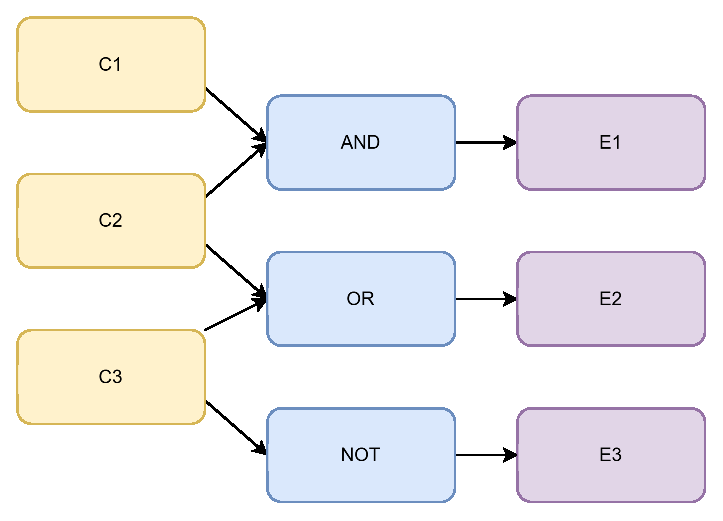
\includegraphics[width=0.7\textwidth,height=190px]{BasicGraph}
	\caption{Basic graph with the corresponding logical operators}
	\label{fig:basic-graph-logical}
\end{figure}

\subsection{Step 3: Applying Boolean Algebra}

Once the logical relationships are established, Boolean algebra is used to simplify and formalize the relationships. For each combination of causes and effects, a corresponding formula is created. This formula will express the exact conditions under which an effect occurs based on the causes.

For instance, if an effect \textbf{E1} occurs only when both \textbf{C1} and \textbf{C2} are true, the corresponding logical formula would be: $ E1 = C1 \land C2 $. This methodology can be applied to the other rules too by the \ref{fig:basic-graph-logical} figure:

\begin{compactitem}
    \item $ E1 = C1 \land C2 $
    \item $ E2 = C2 \lor C3 $
    \item $ E3 = \lnot C3 $
\end{compactitem}

In summary, each effect is equivalent to its connected causes and logical nodes. The Boolean value of the expression determines the Boolean value of the corresponding effect.

\subsection{Step 4: Handling Complex and Nested Conditions}

For graphs with nested conditions or complex dependencies, the transformation involves breaking down the graph into simpler components. Each sub-condition is transformed individually before being combined into the final logical expression.

\begin{figure}[H]
	\centering
	\includegraphics[width=0.8\textwidth,height=190px]{ComplexRule}
	\caption{A complex rule for the nested conditions}
	\label{fig:complex-rule-graph-logical}
\end{figure}

For example, consider the \ref{fig:complex-rule-graph-logical} graph logic: $ (C1 \land C2) \lor (C3 \land \lnot C4) $. This represents a scenario where \textbf{E4} occurs if either both \textbf{C1} and \textbf{C2} are true, or \textbf{C3} is true while \textbf{C4} is false. The transformation results in the following Boolean formula: $ E4 = (C1 \land C2) \lor (C3 \land \lnot C4) $.

This formula captures the decision-making logic of the system by accounting for all relevant conditions.

\subsubsection{Handling Constraints and Dependencies}

In some cases, certain conditions or dependencies in the business logic must also be modeled, such as mutually exclusive outcomes or constraints on the input values. These constraints are incorporated into the logical formulas, ensuring that only valid combinations of causes are tested.

For example, if \textbf{C1} and \textbf{C4} are mutually exclusive, the formula must reflect this: $ C1 \land C4 = false $. This ensures that test cases generated from the formula will not include invalid or contradictory conditions.

This format simplifies complex logic into a more manageable form. Any disjunction that is true will cause the effect to occur. For a disjunction to be true, each element within its inner conjunction must also be true. We will utilize this characteristic moving forward.

\subsection{Step 5: Generating Disjunctive Normal Form (DNF)}

In many cases, the logical formula needs to be converted into Disjunctive Normal Form (DNF) to be used with certain solvers or test generation tools. DNF is a standardized format where the formula is expressed as a disjunction of conjunctions, making it easier to handle by many automated tools.

For example, the expression $ (\lnot C1 \lor C2) \land (\lnot C3 \lor C4) $ can be rewritten in DNF: $ (C1 \land \lnot C3) \lor (C2 \land \lnot C4) $

\subsection{Step 6: Finalizing the Logic in a Decision Table}

Once we reach the DNF of the logical definition, it is ready to be converted into a decision table. This marks the final stage of the logical transformation process and provides a result that is well-suited for the next steps, including test generation.

As previously mentioned, the decision table includes all non-logical nodes, listing the causes and effects in each row. Rules can be created from the transformed logical expression in DNF, forming the columns of the table. Each column represents an impacted effect and all associated causes included in it.

\begin{table}[H]
	\centering
	\begin{tabular}{ | m{0.11\textwidth} | m{0.11\textwidth} | m{0.11\textwidth} | m{0.11\textwidth} | m{0.11\textwidth} | m{0.11\textwidth} | m{0.11\textwidth} | }
		\hline
		\textbf{Nodes} & \textbf{Rule 1} & \textbf{Rule 2} & \textbf{Rule 3} & \textbf{Rule 4} & \textbf{Rule 5} & \textbf{Rule 6} \\
		\hline \hline
		\emph{C1} & 1 & - & - & - & 1 & - \\
		\hline
		\emph{C2} & 1 & 1 & - & - & 1 & - \\
		\hline
		\emph{C3} & - & - & 1 & 0 & - & 1 \\
		\hline
        \emph{C4} & - & - & - & - & - & 0 \\
		\hline \hline
        \emph{E1} & 1 &   &   &   &   &   \\
		\hline
        \emph{E2} &   & 1 & 1 &   &   &   \\
		\hline
        \emph{E3} &   &   &   & 1 &   &   \\
		\hline
        \emph{E4} &   &   &   &   & 1 & 1 \\
		\hline
	\end{tabular}
	\caption{Final decision table at the end of the logical transformation (1 = true and 0 = false) for the figure \ref{fig:basic-graph-logical} and figure \ref{fig:complex-rule-graph-logical}}
	\label{tab:final-decision-table}
\end{table}

Each disjuncts of the DNF entries are translated into a rule (Rule 1, Rule 2, etc...) in the table \ref{tab:final-decision-table}, and the elements of the corresponding conjunction are represented by the values that make the effect true (1).

This provides a complete overview of the effects and the various states that trigger them. This characteristic enables certain test automation tools to generate a set of test cases directly from the table \ref{tab:final-decision-table}.

A well-defined graph enables the decision table to serve as a source for numerous test cases, covering all possible combinations of causes and effects and helping to uncover hidden faults in the system.

\section{Example Conversion}

To illustrate the transformation of a cause-effect graph into logical formulas, let's walk through a simple example. We will take a basic cause-effect scenario and convert it into a set of Boolean expressions and a Decision table that can be used for automated test generation.

\subsection{Step 1: Define the Causes and Effects}

Consider a system where a user must input both a valid username and password to gain access. The cause-effect graph would include the following elements:

\begin{table}[H]
	\centering
	\begin{tabular}{ | m{0.2\textwidth} | m{0.2\textwidth} | m{0.3\textwidth} | }
		\hline
		\textbf{Name} & \textbf{Type} & \textbf{Description} \\
		\hline \hline
		\emph{C1} & Cause & Valid username provided \\
		\hline
		\emph{C2} & Cause & Valid password provided \\
		\hline
        \emph{E1} & Effect & Access granted \\
		\hline
        \emph{E2} & Effect & Access denied \\
		\hline
	\end{tabular}
	\caption{The decision table result of the example after the DNF conversion}
	\label{tab:example-cause-effect-collection-table}
\end{table}

The elements in the table \ref{tab:example-cause-effect-collection-table} will represent the nodes, which will be the primary components of the visualized graph, while the relationships between them will be represented by the logical nodes.

\subsection{Step 2: Establish Logical Relationships}

In this example, the system grants access only if both the username and password are valid. If either the username or password is invalid, access is denied. The cause-effect graph would visually represent these relationships with \textbf{AND} and \textbf{NOT} nodes:

\begin{compactitem}
    \item E1 = C1 AND C2 (access is granted only if both the username and password are valid)
    \item E2 = NOT (C1 AND C2) (access is denied if either the username of password is invalid)
\end{compactitem}

\subsection{Step 3: Representing the Logic in Boolean Form}

Based on the cause-effect graph, we can now convert the relationships into Boolean expressions:

\begin{compactitem}
    \item \textbf{Access granted (E1)}: $ E1 = C1 \land C2 $
    \item \textbf{Access deined (E2)}: $ E2 = \lnot (C1 \land C2) = (\lnot C1 \lor \lnot C2) $
\end{compactitem}

It is evident that the \textbf{E2} formula can be simplified. By applying \emph{De Morgan's law}, the negation is pushed inside the AND operation, transforming it into an OR operation.

\subsection{Step 4: Converting to Disjunctive Normal Form (DNF)}

We would convert the Boolean expressions into DNF. The formula is expressed as a set of AND clauses that are ORed together. In this example, the formula for access denied (\textbf{E2}) is already in DNF: $ E2 = (\lnot C1 \lor \lnot C2) $. It is a disjunction of two single-item conjunctions.

The formula for access granted (\textbf{E1}) can be expressed in DNF by leaving it as a simple conjunction: $ E1 = C1 \land C2 $. However, it is not a disjunction but rather a simplified form of a single-item disjunction.

\subsection{Step 5: Validation the Logical Formulas}

Once the conversion is complete, the generated logical formulas can be validated. These formulas now represent the decision-making logic of the system, ensuring that access is correctly granted or denied based on the inputs.

For instance:

\begin{compactitem}
    \item If both \textbf{C1 = 1} and \textbf{C2 = 1} (valid username and password), \textbf{E1 = 1} (access granted)
    \item If either \textbf{C1 = 0} or \textbf{C2 = 0} (invalid username or password), \textbf{E2 = 1} (access denied)
\end{compactitem}

A decision table can be created from this result as follows:

\begin{table}[H]
	\centering
	\begin{tabular}{ | m{0.2\textwidth} | m{0.2\textwidth} | m{0.2\textwidth} | m{0.2\textwidth} | }
		\hline
		\textbf{Nodes} & \textbf{Rule 1} & \textbf{Rule 2} & \textbf{Rule 3} \\
		\hline \hline
		\emph{C1} & 1 & 0 & - \\
		\hline
		\emph{C2} & 1 & - & 0 \\
		\hline \hline
        \emph{E1} & 1 &   &   \\
		\hline
        \emph{E2} &   & 1 & 1 \\
		\hline
	\end{tabular}
	\caption{The decision table result of the example after the DNF conversion}
	\label{tab:example-final-decision-table}
\end{table}

\subsection{Visualization}

The visualization of the example is straightforward and can be constructed from Step 1 and Step 2. The main elements and their logical relationships define the graph. The next figure \ref{fig:example-visualization-as-graph} shows this.

\begin{figure}[H]
	\centering
	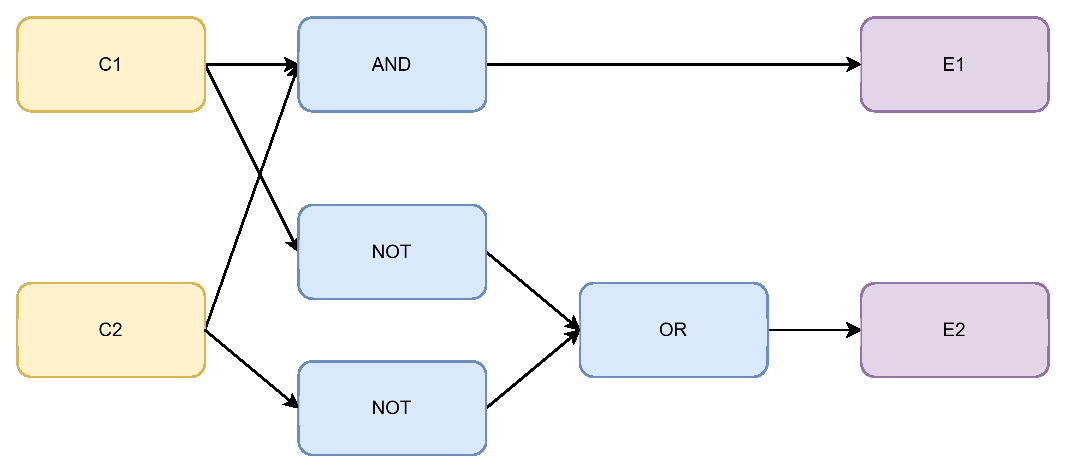
\includegraphics[width=0.8\textwidth,height=160px]{ExampleVisualization}
	\caption{The visualization of the graph for the example.}
	\label{fig:example-visualization-as-graph}
\end{figure}

\section{Importance of DNF}

Converting logical formulas derived from cause-effect graphs into Disjunctive Normal Form (DNF) is a critical step for several reasons, particularly in the context of automated testing and logic-based analysis.

\begin{enumerate}
    \item \textbf{Standardization for Solvers}: Many automated testing tools and satisfiability solvers (SAT solvers) require input in a normal form to function efficiently. DNF provides a standardized structure, making it easier for these tools to process and analyze the logic. From the formulas, the system can leverage these solvers to identify satisfiable inputs, detect inconsistencies, or generate optimized test cases.
    \item \textbf{Improved Computational Efficiency}: DNF reduces the complexity of evaluating logical expressions. It breaks down complex logical relationships into smaller, manageable units (clauses), each of which is a conjunction of literals. These clauses can be evaluated independently, which speeds up the process of checking satisfiability and make the system more scalable.
    \item \textbf{Simplifying the Logic}: DNF inherently simplifies the logical structure by breaking down complex relationships into basic logical operations. This simplification is particularly useful when dealing with intricate business logic, as it makes it easier to understand and debug the logic. Simplified expressions also reduce the likelihood of errors.
    \item \textbf{Compatibility with Other Logical Techniques}: DNF is widely used in conjunction with other formal methods and logic-based techniques, such as model checking and theorem proving. Having the logic represented in DNF allows the system to integrate smoothly with a variety of verification tools and techniques.
    \item \textbf{Convertability to Decision Table}: DNF expressions can be easily converted into a decision table. A well-constructed decision table aids in generating test cases, which helps ensure the correctness of the test subject.
\end{enumerate}

By converting cause-effect graphs into DNF, the system gains efficiency, scalability, and compatibility with existing logic-based tools, ensuring a more rigorous and comprehensive testing approach.

\section{Algorithm for DNF Conversion}

Through transformation, simplification, and optimization, we can convert a logical formula into Disjunctive Normal Form. The process will take a logical formula as input and produce an equivalent logical formula in DNF as output.

\begin{enumerate}
    \item Move negations inward
        \begin{itemize}
            \item Apply \textbf{De Morgan's laws} to push the negations inside:
                \begin{itemize}
                    \item Convert $ \lnot (A \land B) $ to $ \lnot A \lor \lnot B $.
                    \item Convert $ \lnot (A \lor B) $ to $ \lnot A \land \lnot B $.
                \end{itemize}
            \item Continue applying this step until all negations are directly applied to literals.
        \end{itemize}
    \item Distribute \textbf{OR} over \textbf{AND}
        \begin{itemize}
            \item If the formula is in the form $ A \land (B \lor C) $, apply the distribution law to transform it to $ (B \land A) \lor (C \land A) $.
            \item Continue this step recursively.
        \end{itemize}
    \item Simplify the formula
        \begin{itemize}
            \item Remove any duplicate literals within the disjunctions.
            \item Simplify multiple negations on the same literal.
            \item Eliminate any clasuses that are tautological.
        \end{itemize}
\end{enumerate}

By following these steps, the logical formula can be converted to DNF, making it suitable for subsequent processes.

\section{Example of DNF Transformation}

Let's explore a few specific examples of transforming logical formulas into DNF.

\begin{itemize}
    \item $ C1 \land (C2 \lor \lnot C1) $ is an unusual logical expression, but it's not in DNF, so the transformation is necessary. Simplification is possible to $ C1 \land C2 $ form what is now in DNF. It is a disjunction of a single item conjunctions.
    \item $ (C1 \land \lnot C2) \lor (\lnot C1 \land C3) $ is a more complex logical expression. However, because it is a disjunction of conjunctions, it is already in DNF.
    \item $ \lnot (C1 \land C2) $ example is not DNF, so wee need to adjust it. By applying \textbf{De Morgan's law}, we can modify it to $ \lnot C1 \lor \lnot C2 $. This expression is now in DNF, as it is a disjunction of single item conjunctions.
    \item For a more detailed example, consider the formula $ (C1 \lor C2) \land \lnot C3 $. By applying the \textbf{distribution law} (OR over AND), we can transform it into $ (C1 \land \lnot C3) \lor (C2 \land \lnot C3) $, which is now in DNF.
\end{itemize}